\section{Analyse Leitungswiderstand}

Ein weiterer Teilbereich dieser Dokumentation ist die theoretische Analyse des maximal zulässigen\\ Leitungswiderstandes eines Programmierkabels. Dabei wurde mit Hilfe des Simulationsprogramm \glqq LT-Spice\grqq{} ein Ersatzschaltbild eines typischen Programmieraufbaus erstellt.\\

\begin{center}
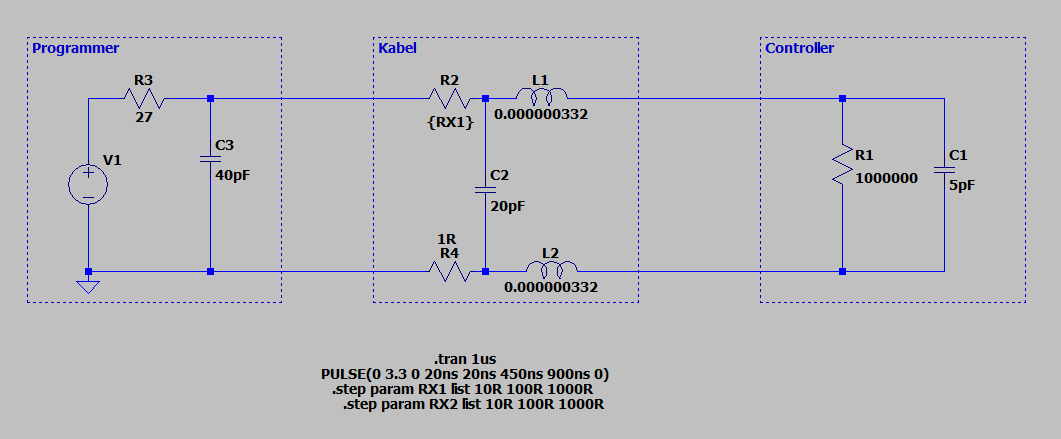
\includegraphics[width=17cm]{Bilder/LTC-SCHALTBILD.png}
\end{center}

Anhand der Datenblätter, welche die Eingangs- und Ausgangseigenschaften von Controller und Programmer der Firma ST beschreiben, wurden Ersatzschaltbilder erstellt. Die passenden Induktivitäten und Kapazitäten des Programmierkabels wurden mit Hilfe eines Online-Rechners für ein 20 cm Kabel berechnet.
\\
\\
Um den Programmiervorgang simulieren zu können gibt die Spannungsquelle V1 ein Rechtecksignal mit ca. 1,1MHz aus. Dies entspricht laut Datenblatt den maximalen Programmiertakt eines ST-Link Programmer. Die zeitliche Dauer einer Signalflanke wurde dabei mit ca.20ns kalkuliert.
\\
\\
Bei der Betrachtung der Signalflanken über Programmer und Controller mit 10R, 100R und 1000R Leitungswiderstand, wurde mir persönlich nicht sofort klar, warum ein geringer Leitungswiderstand so wichtig für den Programmiervorgang ist. 

\begin{center}
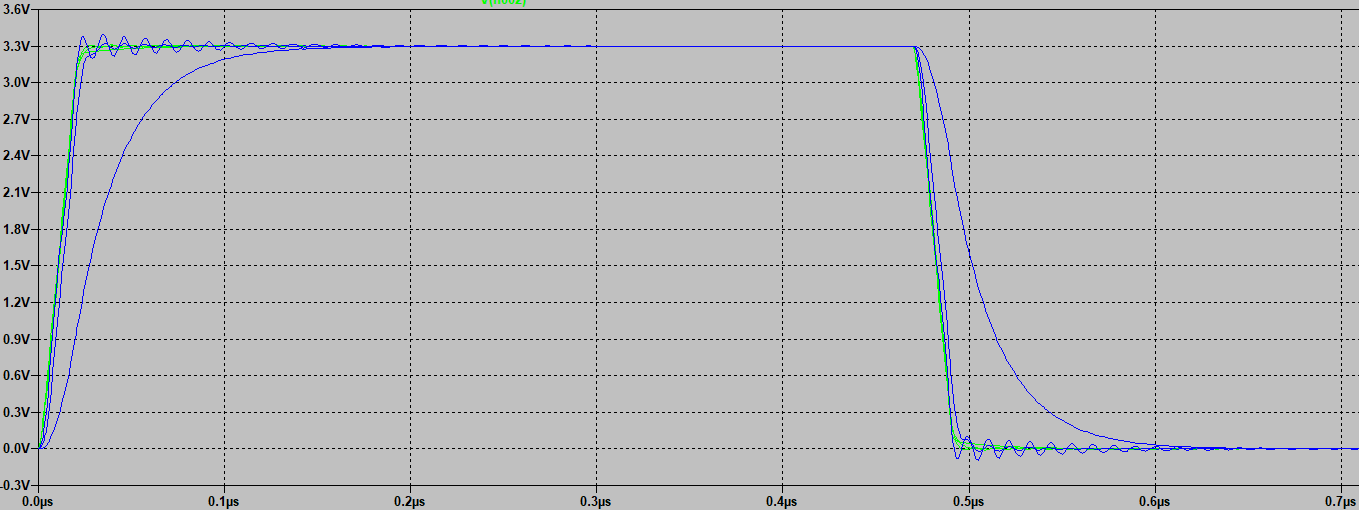
\includegraphics[width=17cm]{Bilder/LTC-SIGNALVERLAUF1.png}
\end{center}

\newpage

Eine differenzielle Messung zwischen Programmer und Controller mit 10R, 100R und 1000R Leitungswiderstand  zeigt den Spannungsunterschied zwischen den beiden Punkten zur selben Zeit. Hierbei zeigt sich, dass während einer Signalflanke kurzzeitig zwischen Programmer und Kontroller ein Potentialunterschied auftritt. Dieser wird mit steigenden Leitungswiderstand größer. Der kleinste Ausbruch tritt bei einem Leitungswiderstand von 10R auf.


\begin{center}
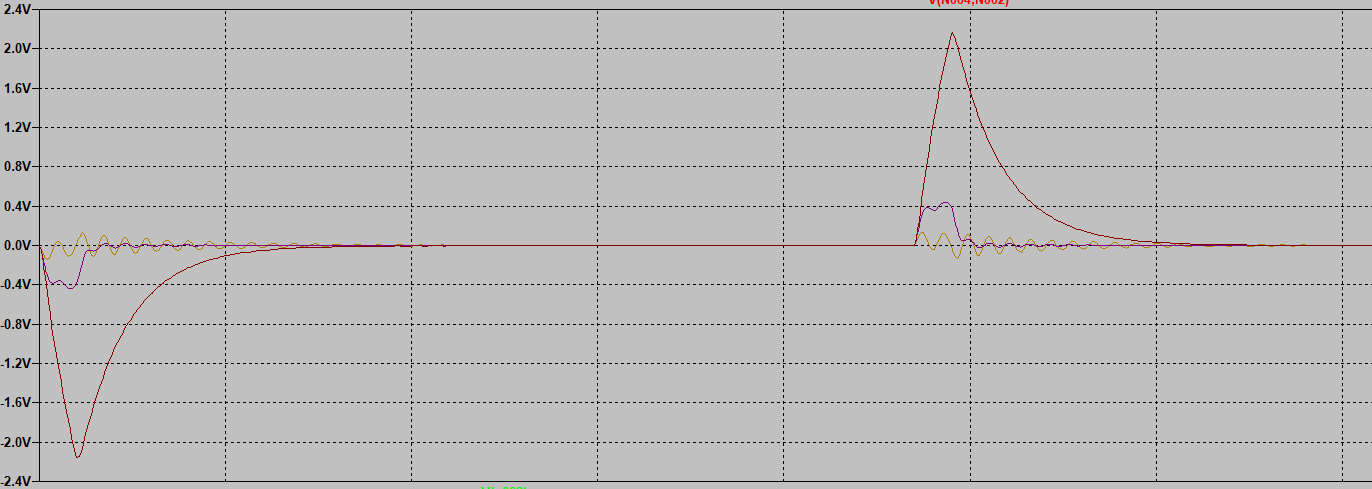
\includegraphics[width=17cm]{Bilder/LTC-SIGNALVERLAUF2.png}
\end{center}

Hierbei handelt es sich um parasitäre Effekte. 
\\
Sie sind unerwünscht und entstehen durch die physikalischen Eigenschaften der Bauelemente. Besonders bei hochfrequenten Anwendungen stellen diese Effekte ein großes Problem dar.
\\
Durch elektrische und magnetische Felder zwischen zwei Punkten können andere Leitungen gestört werden. Dabei kann es zu Datenübertragungsfehlern kommen.
\\
\\
Aus meiner Simulation geht hervor, dass die parasitären Effekte bis zu einem Leitungswiderstand von 10R vernachlässigbar sind. Das von mir entwickelte Prüfgerät wurde daher auf einen Grenzwert von 5R eingestellt. 
